\documentclass{standalone}
\usepackage{tikz}

\usetikzlibrary{calc,fadings,arrows.meta}
\tikzfading[name=fade l,left color=transparent!100,right color=transparent!0]
\tikzfading[name=fade r,right color=transparent!100,left color=transparent!0]
\tikzfading[name=fade d,bottom color=transparent!100,top color=transparent!0]
\tikzfading[name=fade u,top color=transparent!100,bottom color=transparent!0]

\definecolor{red}{HTML}{972e21}
\definecolor{yellow}{HTML}{ebb83f}
\definecolor{blue}{HTML}{5e7fbf}
\definecolor{green}{HTML}{5fd94e}


\begin{document}
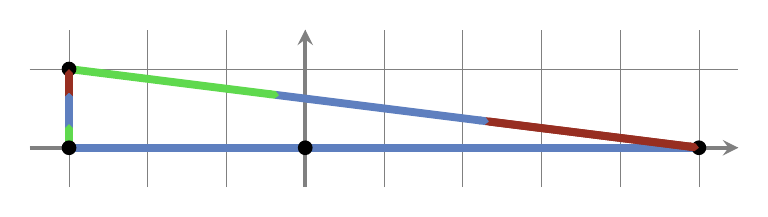
\begin{tikzpicture}[every path/.style={line width=0.05cm}]
  %\clip (-3.5,-0.5) rectangle (5.5,1.5);
  \draw[step=1cm,gray,very thin] (-3.5, -0.5) grid (5.5, 1.5);
  \draw[gray,-stealth] (-3.5,0) -- (5.5, 0);
  \draw[gray,-stealth] (0,-0.5) -- (0, 1.5);
  
  %\fill[white,path fading=fade u] (-3.5,-1) rectangle (6,-0.5);
  %\fill[white,path fading=fade d] (-3.5,2) rectangle (6,1.5);
  %\fill[white,path fading=fade r] (-3.5,-1) rectangle (-3.5,2);
  %\fill[white,path fading=fade l] (5.5,-1) rectangle (6,2);
  
  \begin{scope}[every path/.style={line width=0.1cm}]
  	\draw[color=blue] (-3,0) -- (5,0);
  	
  	\draw[-{Triangle Cap[]},color=red,shorten <=-0.05cm] (-3,0.7) -- (-3,1);
  	\draw[-{Triangle Cap[]},color=blue,shorten <=-0.05cm] (-3,0.3) -- (-3,0.7);
  	\draw[-{Triangle Cap[]},color=green] (-3,0) -- (-3,0.3);
  	
  	
  	\draw[-{Triangle Cap[]},color=red,shorten <=-0.05cm] (2.333,0.333) -- (5,0);
  	\draw[-{Triangle Cap[]},color=blue,shorten <=-0.05cm] (-0.333,0.666) -- (2.333,0.333);
  	\draw[-{Triangle Cap[]},color=green] (-3,1) -- (-0.333,0.666);
  \end{scope}
  
  \node (p1) at (-3,0)[circle,fill,inner sep=0.066cm]{};
  \node (p2) at (0,0)[circle,fill,inner sep=0.066cm]{};
  \node (p3) at (5,0)[circle,fill,inner sep=0.066cm]{};
  \node (p4) at (-3,1)[circle,fill,inner sep=0.066cm]{};
  
  \begin{scope}[every path/.style={line width=0.1cm}]  	
  	\draw[-{Triangle Cap[]},color=red] (-3,0.7) -- (-3,1);
  	%\draw[color=green,line cap=round,shorten <=0.1cm,shorten >=0.1cm] (-3,0) -- (-3,0.3);
  	
  	\draw[-{Triangle Cap[]},color=red] (2.333,0.333) -- (5,0);
  	%\draw[color=green,line cap=round,shorten <=0.1cm,shorten >=0.1cm] (-3,1) -- (-0.333,0.666);
  \end{scope}

\end{tikzpicture}
\end{document}

% For 2nd query: 33s to get from 1 to 3
% ans = 19.05l = 19.03s of acceleration.
% fuel/edge ~ sqrt(length)
% lengths = 1, sqrt(65)=sqrt(1^2+8^2)
% sum(sqrt(len)) = 1+sqrt(sqrt(65)) = 3.839
% fuel for edge 1: t1= 1/3.839 * 19.05 = 4.96
% fuel for edge 2: t2= 65**0.25/3.839 * 19.05 = 14.09
% edge 1 accel&decel: 1/2 (t1/2)^2 = t1^2/8 = 3.07
% edge 2 accel&decel: 1/2 (t2/2)^2 = t2^2/8 = 24.8
%
